%*******************************************************************************
%****************************** Second Chapter *********************************
%*******************************************************************************

\chapter{Social networks and social support}

\label{chap:Utility_support}
\graphicspath{{Chapter3/plots/} {Chapter3/plots}}
\begin{quote}
    \textit{''The original idea of the web was that it should be a collaborative space where you can communicate through sharing information... In an extreme view, the world can be seen as only connections, nothing else.``} - Tim Berners Lee\cite{berners2001weaving} 
\end{quote}
Attention budgets pretty much govern how we as consumers interact with online social networks. It has been shown that the dearth of this budget, promotes an engagement behaviour that prioritizes perceptive features and immediacy in the content. The scrolling user interface of platforms like Instagram and Facebook, allow mere seconds to decide whether a particular content is worth the user's attention~\cite{eikelboom2017irresistible}. 
However, there is a whole breed of online social networks, which aim at bringing the offline sense of networking, online. These networks are mostly designed around a specific purpose like technical discussions\footnote{\url{www.stackoverflow.com}}, subject specific questions\footnote{\url{www.stackexchange.com}} or simply around hobbies like knitting\footnote{\url{www.ravelry.com}} or art\footnote{\url{www.artween.com/}}. These communities embody the true essence~\cite{berners2001weaving} of the internet, in that they strive at making geographical distance secondary, to the act of social networking and information sharing.

In the context of this dissertation, I wanted to know how signatures of a perceived entity like social support,  manifests on these formal social networks. More specifically I have followed the DIKW framework, to look at the signatures of perceived \textsl{social support} on communities designed around users who have underwent or are undergoing physical or mental distress. According to the seminal work by Shumaker and Brownell~\cite{shumaker1984toward}, social support is defined as \textsl{``an exchange of resources between two individuals perceived by the provider or the recipient to be intended to enhance the well-being of the recipient.''}
Under this construct , these communities are apt Petri dishes to study the signatures of the online social support. Once you could quantify the social support signatures in terms of computable metrics, platforms could then empower the participants of these communities and design interventions to curb negative behaviour like trolling. The first step to this goal, was to understand the structure and utility of these communities. More over, having a primer on these communities would help the reader get an idea about the methods developed over the course of this dissertation. 

\section{Online health communities}
Recent work has proposed that online communities have the potential to influence health and health care sectors. Recent studies have suggested that the participation of people with long-term conditions (LTCs) in online communities (1) improves illness self-management~\cite{allen2016long}, (2) produces positive health-related outcomes\footnote{\url{https://bit.ly/2FLcs1F}}~\cite{mo2012developing,pendry2015individual} , (3) facilitates shared decision-making with health care professionals~\cite{bartlett2011investigation,izuka2017stroke}, and (4) may even reduce mortality~\cite{hobbs2016online}.

There is also evidence that self-management support interventions can reduce health service utilization~\cite{panagioti2014self,taylor2014rapid}. This is especially a crucial point as the world health services are facing the brunt of an ageing population.

Online communities have experienced an upsurge in popularity among people with chronic respiratory conditions such as cystic fibrosis~\cite{kirk2016exploration}, asthma~\cite{stewart2011online}, pulmonary hypertension~\cite{matura2013virtual} and chronic obstructive pulmonary disease (COPD)~\cite{wentzer2013narratives}. More than 15 million people in England suffer from a long-term condition or disability, and they account for at least 50 percent of all general practitioner appointments\footnote{\url{https://bit.ly/2EVFs9v}}. Thus, assessing how these online communities function, evolve and provide perceived support, can have important implications for health care sector. More so, understanding the dynamics of these online communities, have actual repercussions on how the platforms that host them, could become a better resource of self-management of LTCs.

%This form of “user-led self-management” of LTCs bears similarities with the “expert patient” model, an approach to self-management of LTCs produced by the United Kingdom (UK) Department of Health in 2001 [16]. Evidence of the effectiveness of conventional off-line self-management programs based on the expert patient model, though, has been weak [17]. Clinic-based self-management programs often failed because of: (1) lack of awareness and engagement among patients and staff, (2) failure to consider low health literacy or cultural norms, (3) lack of attention to the need for family and social support, and (4) a fragmented approach to the provision of health and social care [18]. Although online health communities can be seen as an extension of the expert patient model, network effects, in addition to the online disinhibition effect [19], make them a distinct and unique complex intervention mechanism.

On average, one in four people with an LTC who use the Internet tries to engage online with others with similar health-related concerns~\cite{fox2011social}. In particular, it has been suggested that the value of participating in an online community lies in the possibility of gaining access to a range of people and resources quickly, easily~\cite{armstrong2000real}, and anonymously~\cite{pendry2015individual}, as well as obtaining tailored information and emotional support~\cite{ali2015online,de2017adolescents,shoebotham2016therapeutic,coulson2005receiving,de2016stroke}. However, most of this evidence comes from qualitative studies, whereas only recent years have witnessed an increasing interest in quantitative assessments of online communities as intervention mechanisms [28-33]. Recent studies have been concerned with the users’ unequal contributions and engagement patterns, and with the role of superusers. However, the contribution of superusers to the sustainability of online health communities and their structural properties remains mostly unclear.

The potential future integration of online health support systems with formal health care provision should be underpinned by a better understanding of how they are used and by evidence of their effectiveness. Indeed, as suggested by the Medical Research Council~\cite{Craiga1655}, integrating online support systems with the more traditional health care provision would require the identification and comparative assessment of potential alternative intervention mechanisms.

%An expanding body of literature concerned with social network analysis has examined the structural patterns of relations among interacting actors and the social mechanisms that enable them to gain access to valuable resources [35]. There is also increasing evidence that network approaches can be applied to understanding the users’ “expertise” [36], their interactions, and network effects on health-related outcomes in online health communities [37,38]. Uncovering the mechanisms underlying the formation of successful social networks requires a study of how online connections among people, namely the social ties or links, emerge and evolve, and how groups of individuals gradually grow in membership and become interconnected with one another. These processes of tie creation and group formation in online patients’ communities are still mostly unexplored [1].
%In this study, we performed a network analysis of the structure and dynamics of two online communities of people with LTCs. We chose the Asthma UK and the British Lung Foundation (BLF) communities as an exemplar of such communities because their users typically suffer from chronic respiratory conditions. In particular, while Asthma UK users typically suffer from a respiratory condition characterized by variable and recurring symptoms, BLF users represent a more heterogeneous population of participants affected by different diseases linked to chronic symptoms of breathlessness (eg, COPD, pulmonary fibrosis, cystic fibrosis, and lung cancer).

In this study, we aim to uncover and understand how these communities function and evolve, and the role that some users have in maintaining integration and cohesion. Ultimately, this study provides evidence for gauging the effectiveness of different interaction patterns, the users’ structural positions and their potential for enhancing and sustaining health online communities as a form of scalable self-management support interventions. 
The key research questions I attempt to answer are : 
\begin{itemize}
    \item What are the structural dynamics of users on these communities ? 
    \item Are there particular users who are more poised to be agents of social support than others? 
    \item How resilient are these communities? 
\end{itemize}


\section{Dataset and properties}
The data was collected from HealthUnlocked\footnote{\url{http://www.webcitation.org/70Y10rppl}}, the online platform provider of the Asthma UK and British Lung Foundation communities. Registered users can choose to either write posts publicly or send private posts to one another. In the latter case, posts are shared between 2 users only, whereas when posts are written publicly, a large number of users can become connected through threads of posts. A thread is a series of posts made on one root post, as a response to the root, or as a response to one of the responses to the root. This tree-like structure of posts can evolve indefinitely between posters. 
Only posts that were shared publicly were collected and analyzed. For this study, user identifiers (IDs) were anonymized by the HealthUnlocked platform, and no demographic information was collected. 
The data set included posts and their metadata (ie, the anonymized user ID numbers), user roles (eg, user, administrator, or moderator), date of posting, the hierarchical level of the post within the corresponding thread, and the dates in which the users joined and left the community. Both communities were moderated, and HealthUnlocked moderators (identified through metadata linked to posts) were included in the analysis to assess their contribution and compare it with other users. Online communities on the HealthUnlocked platform benefit from additional functionalities compared to other online forums, such as built-in patient groups that moderate the content. In particular, the content accessed by users is tailored to their interests, and profiles highlight users’ condition, chosen community, medications and treatments they use or find interesting. No data were collected on participants’ characteristics, though only people declaring themselves to be older than 16 years were permitted to create an account and take part in the online communities. Table \ref{table:jmirData} summarizes the salient features of the dataset used for this work. 


\begin{table}[htb!]
\centering
\begin{tabular}{ |p{5cm}|p{5cm}|p{5cm}| }
    \hline
    \multicolumn{3}{|c|}{Dataset Properties} \\
    \hline
    \hline
     \textbf{Property} & \textbf{AsthmaUK} & \textbf{British Lung Foundation} \\
    \hline
    \hline
     Time span of data   	& 02/03/2006-06/09/2016    	& 13/04/2012-06/09/2016 \\
    \hline
     Total Time (weeks)  	& 548						& 230 \\
    \hline
     Total number of posts	& 32,780					& 875,151 \\
    \hline
     Percentage of posts with at-least 1 reply & 87.3\%			& 93.1 \% \\
    \hline
     Total number of users &	3345					& 19,837 \\
    \hline
     Users who contributed > 1 posts (\%n) & 1053 (31.5)  & 7814 (39.4) \\
    \hline
     Users who contributed exactly 1 post(\%n) & 331 (31.4) 722 & 1186 (15.2) \\
    \hline
     Registered users who never posted (ie, lurkers), n (\%) & 2292 (68.5) & 12,023 (60.6) \\
    \hline
     Number of posts per user, $\mu(\sigma)$ & 14.2 (55.0) & 66.9 (75.1) \\
    \hline
    Number of posts per users who posted >1, median (min - max) & 5.1 (2-1068) & 8.0 (2-8947) \\
    \hline 
    Number of posts per users who posted >1, mean (SD) & 20.4 (65.6) & 88.1 (458.6) \\
    \hline
    Posts contributed by top 1\% users by activity, n (\%) & 10,457 (31.9) & 426,198 (48.7) \\
    \hline 
    
    \hline
\end{tabular}
\caption{The summary of salient attributes of the data used for this work}
\label{table:jmirData}
\end{table}

The data sets span, respectively, 10 years for the Asthma UK and 4 years for the BLF communities (see Table 1).

Despite the shorter time span, as a result of the larger number of users, the number of posts in the BLF community was higher than in Asthma UK, namely 875,151 compared to 32,780 respectively. Moreover, BLF users wrote a higher number of posts per user and were connected with a higher number of other users when compared with people in the Asthma UK forum (see Figure 2). In both communities, 60\%-70\% of registered users wrote no posts (ie, they were lurkers). Users who wrote more than one post contributed with a median of 8 (range 2-8947) and 5 (range 2-1068) posts in the BLF and Asthma UK communities, respectively.

The number of official moderators among the highly active users was negligible; there were no moderators in the top 5\% contributors to BLF and only 2 in the top 5\% for Asthma UK. Thus, our network analysis predominantly reflects content originated from registered users.

When classified according to posting activity (ie, number of posts written to the forum), the top 5\% users contributed to a substantial proportion of all posts: 58\% and 79\% in the Asthma UK and BLF communities, respectively. Superusers were those who made a high number of connections with other users in both Asthma UK and BLF communities (see nodes of large size in Figure 2). Asthma UK superusers made a lower number of connections than BLF ones. The posting activity of these superusers will be analyzed in more detail in subsequent sections.


\section{Abstraction: Graphs}
From this raw data of user posts and their thread structure, I generated a graph abstraction which abstracts our users as nodes of the graph and edges as exchange of messages between two users. More formally imagine a directed graph $G(V,E)$ involving a set of users $V_i\forall i \in N$ where N is the total number of users interacting on a health community. For every message exchanged between a user $i$ and a user $j$ we create an edge $E_{ij}$. The complete community would form a global graph based off total interactions between all pairs of users which we call a global graph $G_g$. Similarly we may decide to only consider the users and messages exchanged across one particular thread discussing a particular issue. Such a graph is called a thread graph $G_t$.

\begin{figure*}[!ht]
    \centering
    % \hspace*{-5mm}
    \subfloat[]{
        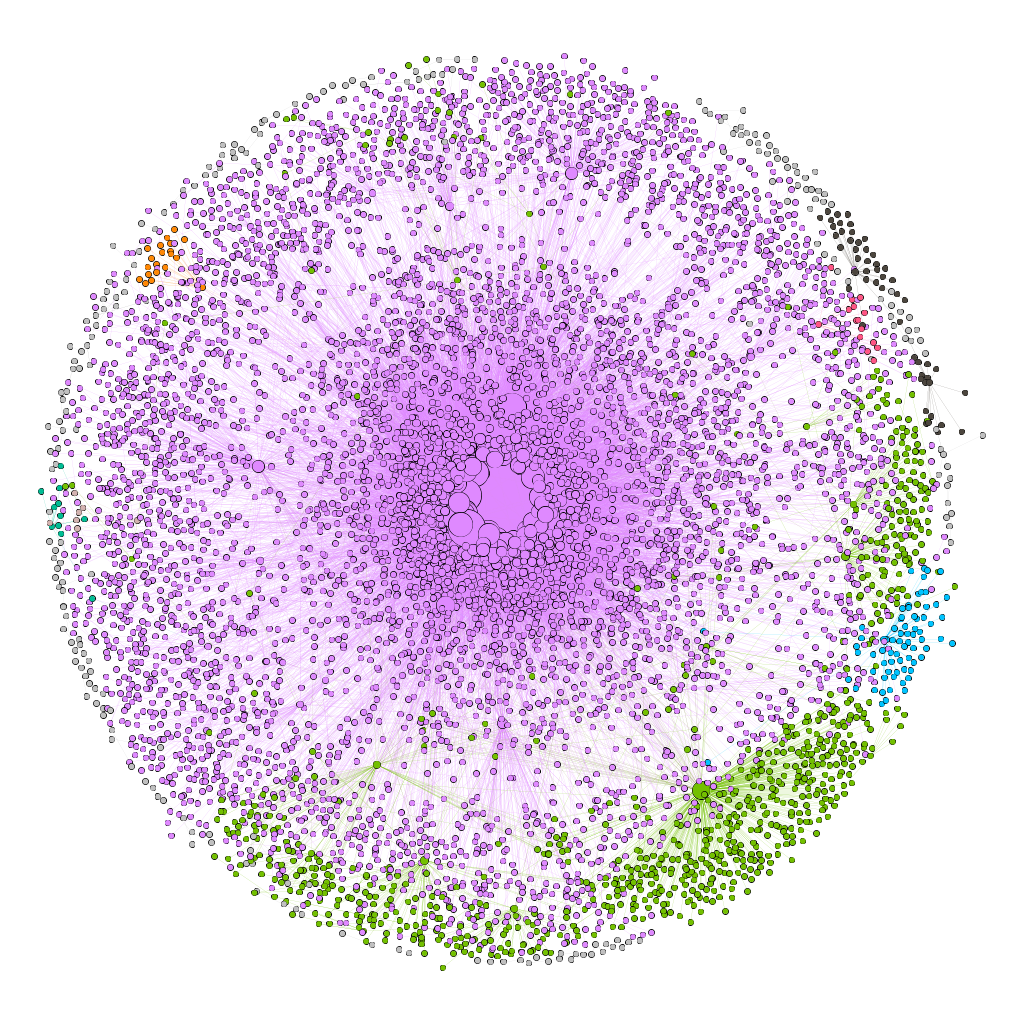
\includegraphics[width=0.5\textwidth ]{BLFWhole.png}
        \label{fig:BLF_graph}
    }
    \subfloat[]{
        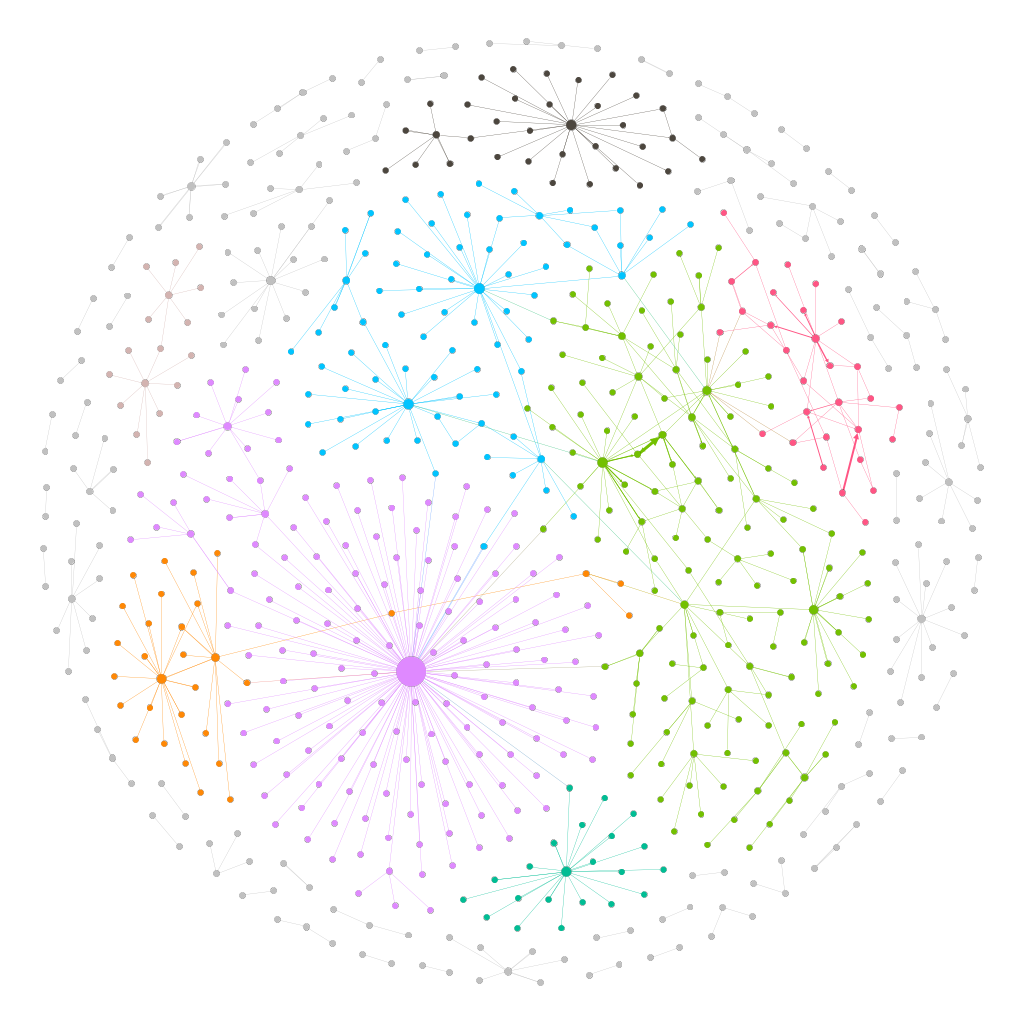
\includegraphics[width=0.5\linewidth ]{AsthamaWhole.png}
        \label{fig:Asthma_graph}
    }
    \caption{Global graphs prepared from Asthama UK community\ref{fig:Asthma_graph} and BLF community\ref{fig:BLF_graph}. The size of the node corresponds to the degree of the node and the color corresponds to the community membership }
\end{figure*}

These graphs are the temporal abstractions of how users interacted on the community either around a particular query (Thread graphs) or over all as a part of the bigger community (Gobal graph). To understand the behaviour of these users, we evaluate several metrics on these graphs to understand the utility of these communities in terms of activity of sharing and support. In the context of this work, we define support as an exchange of information on account of a query.

\subsection{Activity Metrics}
To calculate the activity patterns of users on these forum, we first work with the most basic of proxies, which is the weekly/daily activity. It is the amount of messages exchanged over a community in a given period of time across the whole life cycle of the data. This is a good metric for the vitality of the community. Another metric to look at is messages exchanged per user per week. This gives an idea of how active an average user is on the community in a given time period. From these basic analysis, it was quite evident that the BLF community was more active of the two. 

\begin{figure}[!ht]
    \centering
    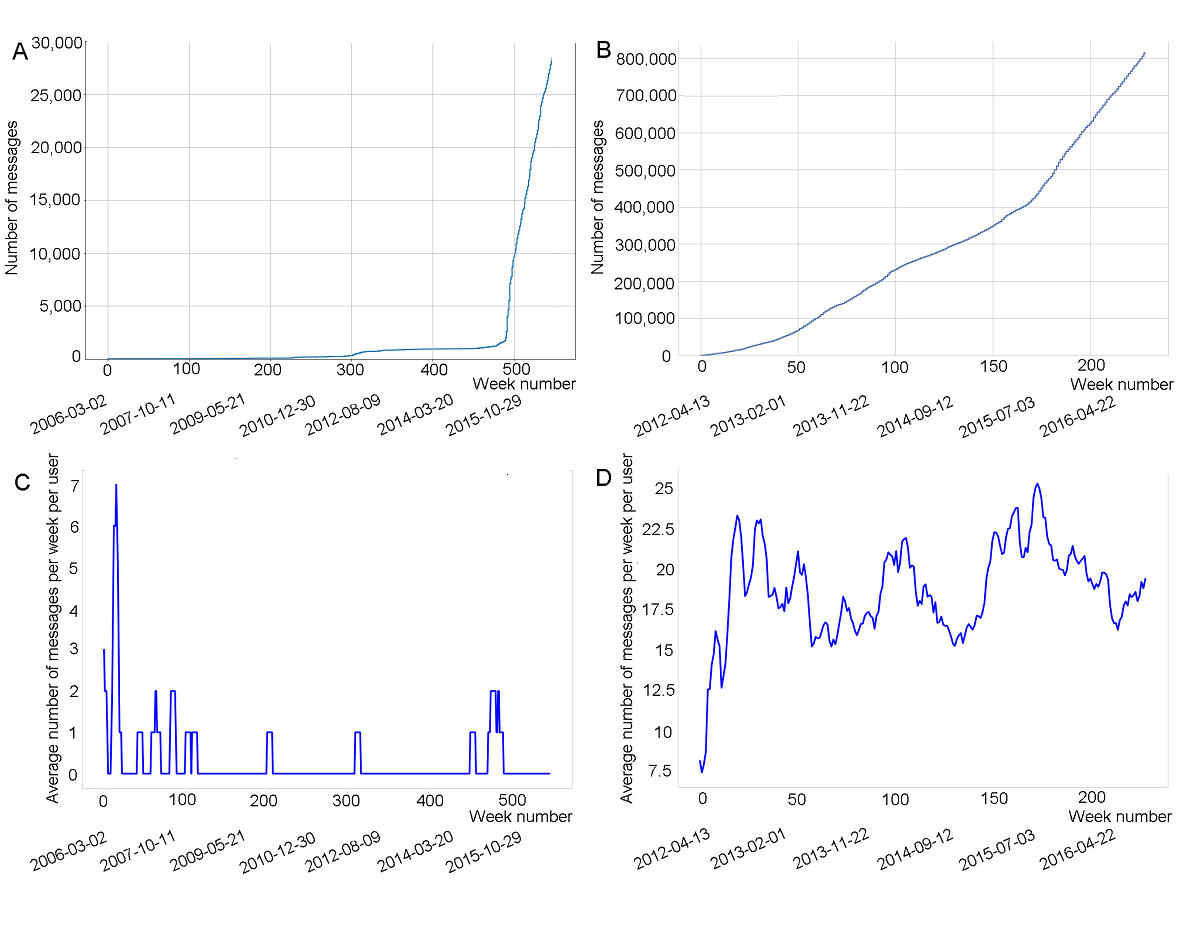
\includegraphics[width=\textwidth ]{Activity.png}
    \label{fig:activity}
    \caption{Cumulative distributions of the number of posts as a function of time (weeks) within the Asthma UK (A) and the British Lung Foundation (B) communities. Calendars dates are reported below week numbers. Panels C and D illustrate the average number of posts per user per week within Asthma UK and British Lung Foundation, respectively}
\end{figure}

\subsection{Community resilience}
From table\ref{table:jmirData}, it is evident that a minority of users are generating a bulk of data on these communities. E.g. the top 1\% users by activity contributed 32\% posts to AsthamaUK community. Such level of activity makes these users extremely important in understanding the dynamics of support on these communities. For this reason I test the resilience of both these communities by progressively removing the most highly connected nodes from the network and testing the collapse of connectivity in the network. This is done by first sorting the nodes by the degree of the network. Then I progressively remove the top 2\% nodes of the nodes in the network and then calculating the size of the weakly connected component as a fraction of original size. 

\section{Activity patterns of users}

\begin{figure}[!ht]
    \centering
    % \hspace*{-5mm}
    \subfloat[]{
        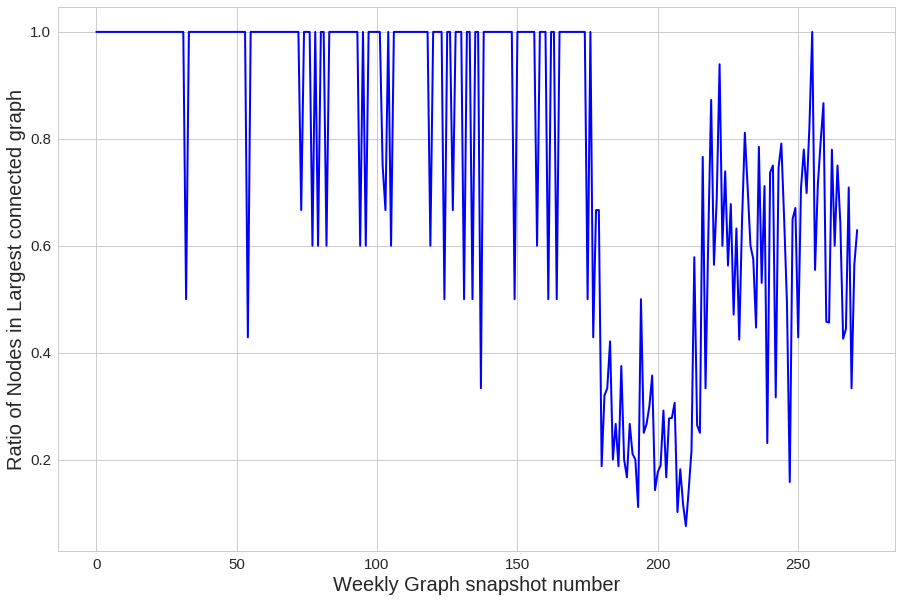
\includegraphics[width=0.5\textwidth ]{ConnectedComponent_weekly_ashtma.png}
        \label{fig:lcc_asthma}
    }
    \subfloat[]{
        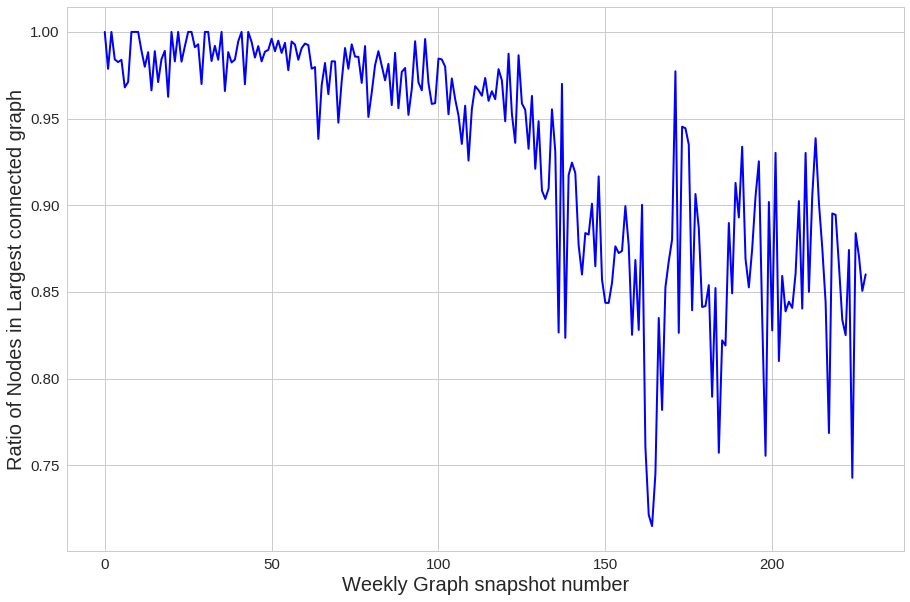
\includegraphics[width=0.5\linewidth ]{weekly_largest_component_BLF.png}
        \label{fig:lcc_blf}
    }


        \subfloat[]{
        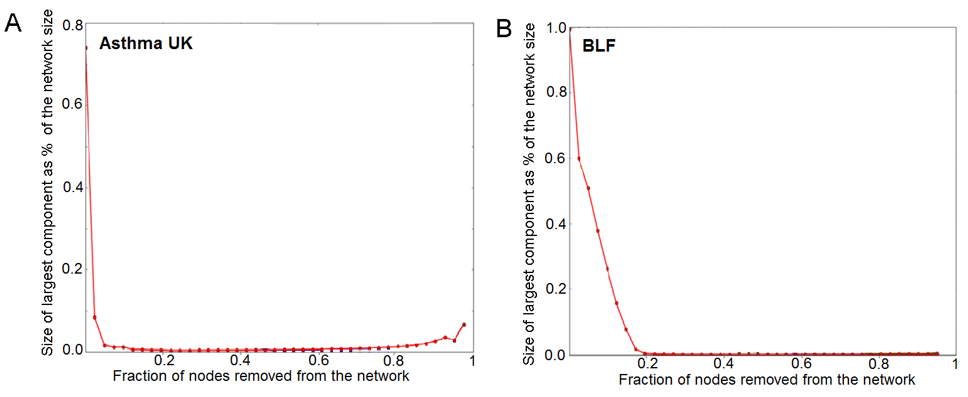
\includegraphics[width=\textwidth ]{jmirSensitivity.png}
        \label{fig:sense_asthma}
    }
    \caption{Fraction of users that are part of the largest component as a function of time (weeks) for Asthma UK \ref{fig:lcc_asthma} and the British Lung Foundation \ref{fig:lcc_blf}. Sensitivity analysis: targeted removal of nodes (users) starting from the most connected ones within Asthma UK \ref{fig:sense_asthma} and the British Lung Foundation. }
\end{figure}


The “rich-club” coefficient is a metric designed to measure the extent to which well-connected users tend to connect with one another to a higher degree than expected by chance [43]. To this end, for each value k of a node’s degree (ie, the number of other users a given user is connected with), we computed the ratio between the number of actual connections between nodes with degree k or larger and the total possible number of such connections [47]. We then divided this ratio by the one obtained on a corresponding random network with the same number of nodes and degree distribution (ie, the probability distribution of the degrees over the whole network) as the real network, but in which links were randomly reshuffled between nodes. Thus, the rich-club coefficients may take values lower or higher than 1, depending on whether the real network has a higher or lower tendency to coalesce into rich clubs than randomly expected. In particular, networks that display a high rich-club coefficient (ie, greater than 1) are also said to show a “rich-club effect,” namely the tendency to organise into a hierarchical structure in which highly connected nodes preferentially create tightly knit groups with one another, thus generating exclusive clubs of (topologically) rich nodes, as illustrated in previous work [48].

In our study, superusers were defined according to their cumulative activity over the entire observation period. In total, we identified 400 superusers. To uncover how many superusers were active within each week, we detected how many unique users, among the 400 identified over the entire period, were active within that time window.

Following Zhang et al [36], the “z-score” was used as a proxy for users’ expertise. According to this measure, replying to many questions suggests one’s expertise, while asking questions indicates lack of expertise. In our analysis, we treated anyone starting a thread as a help-seeker, and anyone commenting on the thread as a help-giver [36]. Accordingly, the proposed z-score aims to capture the combined help-seeking and help-giving patterns. To this end, for each user, we measured how many standard deviations the observed total number of the user’s help-giving posts lies above or below the expected number of help-giving posts for the whole system. We extended the approach proposed by Zhang et al by empirically assessing the probability of posting and answering a question across all users over the entire observation period. In the BLF community, we found that the probability of answering is Pa=2/3, while the probability of posting is Pq=1/3. We assumed a Bernoulli process of posting an answer or a question to the forum, with probabilities defined as above. The z-score for a given user i was calculated according to equation (a) in Figure 1, where ai refers to the total number of answers user i posted to the forum, qi is the total number of questions user i asked in the forum, and ni=ai +qi is the total number of messages posted by user i.
To obtain $Zscore_i$, let us define a random user that posts the same total number of messages nrandom to the forum as user i (ie, nrandom=ni). We would expect this random user to post an average number of answers to the forum given by equation (b). Plugging in the value of $Pa=2/3$, we obtained equation (c). Similarly, we would expect the random user to post answers with a standard deviation given by equation (d). Plugging in the value of $Pa=2/3$, we obtained equation (e). To measure how many standard deviations above or below the expected random value a user i lies, we then computed Zscorei according to equation (f). Plugging in the values of $\mu_{random}$ and $\sigma_{random}$, we obtained equation (g). Finally, by substituting $ni=ai +qi$, we obtained equation (h). 


\subsection{Activity}

The cumulative number of messages posted grew uniformly over time in the BLF community. By contrast, in 2015, the Asthma UK forum witnessed a substantial increase in posting activity, at a time coinciding with its move to the HealthUnlocked platform (see Figure 3A and B). This increase in activity can be attributed to the online community functionalities offered by HealthUnlocked, as described in the Methods.

The number of posts per user per week oscillated around a decreasing and an increasing trend (Figure 2C and D), while at the same time the number of posts always went up over the study period (Figure 1A and B). This suggests that there were intervals of time during which the rate of increase in new users was larger than the rate of increase in total posts. Moreover, in the Asthma UK forum users wrote according to two time patterns—they posted at an interval of 1-20 days or 6 months (Figure 4A), while those in the BLF community at an interval of 2 days (Figure 4B).

As more users joined the communities and connected to one another through online posts, distinct groups of connected users started to emerge. These groups, called network components (see Textbox 2), have fundamental implications for the effectiveness of processes of network dynamics such as information diffusion [49]. In a relatively short period, both communities underwent the formation of the “largest component” of connected users, namely a connected subset of users whose size increasingly outgrew the size of all other components (see Figures 1 and 4, and Multimedia Appendices 1 and 2). The largest connected components in both communities included 60%-100% of users.

Figure 5 suggests that, as time went by, the number of forum participants and their posting activity increased, and the proportion of users who were part of the largest components decreased. This finding was expected because the number of posts also rose exponentially, yet at times at a lower rate than the one at which new users joined the communities (see Figure 1C and D). It, therefore, became more difficult for the network to self-organize into a connected component that would include 100\% of the users. Figure 5A also shows that around week 450, when the forum moved to the HealthUnlocked platform, a larger fraction of users began to join the largest connected component, thus highlighting the role that the new online platform played in strengthening the connectedness of the network (see also Figure 3A and B).

\section{Propensity to help} 

\begin{figure}[!ht]
    \centering
    % \hspace*{-5mm}
    \subfloat[]{
        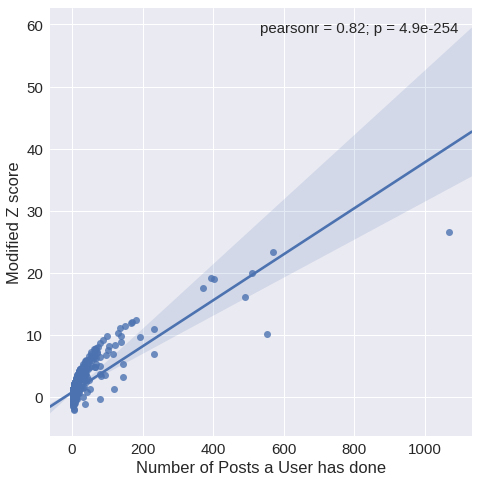
\includegraphics[width=0.5\textwidth ]{ModifiedZScore_asthma.png}
        \label{fig:zscore_asthma}
    }
    \subfloat[]{
        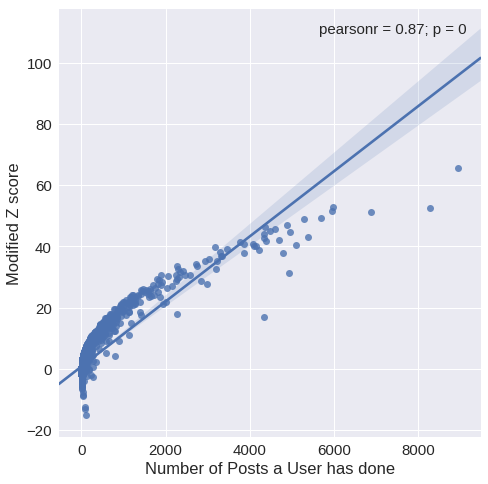
\includegraphics[width=0.5\linewidth ]{Modified_ZScore.png}
        \label{fig:zscore_blf}
    }
    \caption{  }
\end{figure}


\section{Not like conventional networks: Anti-rich club effect}
\begin{figure}[!ht]
    \centering
    % \hspace*{-5mm}
    \subfloat[]{
        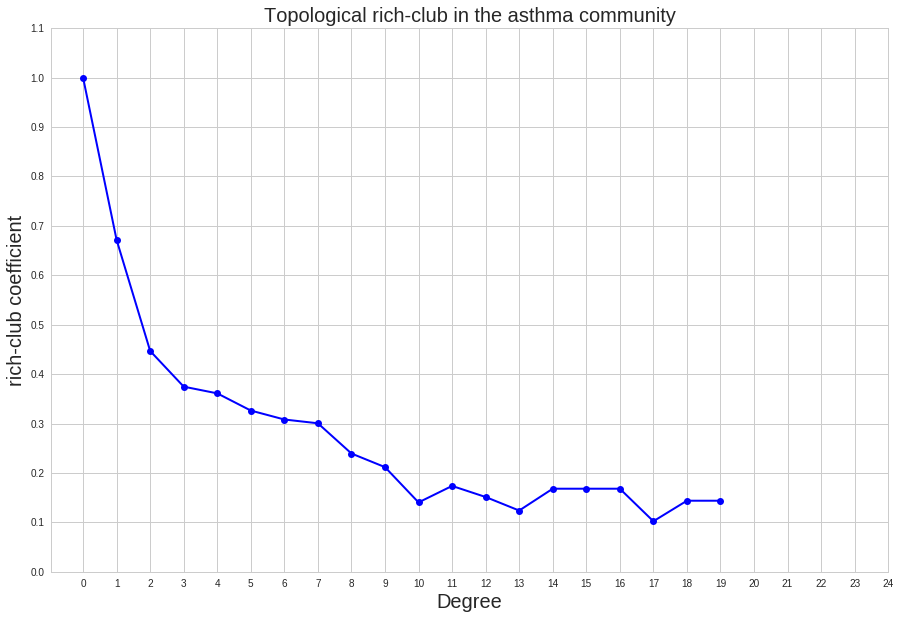
\includegraphics[width=0.5\textwidth ]{RichClub_asthma_truncated.png}
        \label{fig:rich_asthma}
    }
    \subfloat[]{
        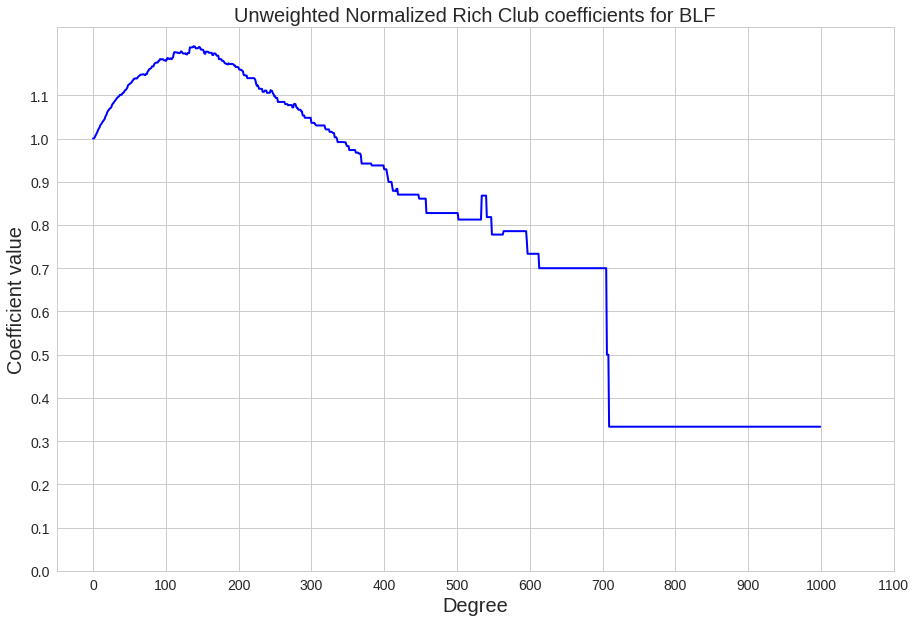
\includegraphics[width=0.5\linewidth ]{RichClub_BLF_truncated.png}
        \label{fig:rich_blf}
    }
    \caption{  }
\end{figure}

\section{ Support is contagious }

\begin{figure}[!ht]
    \centering
    % \hspace*{-5mm}
    \subfloat[]{
        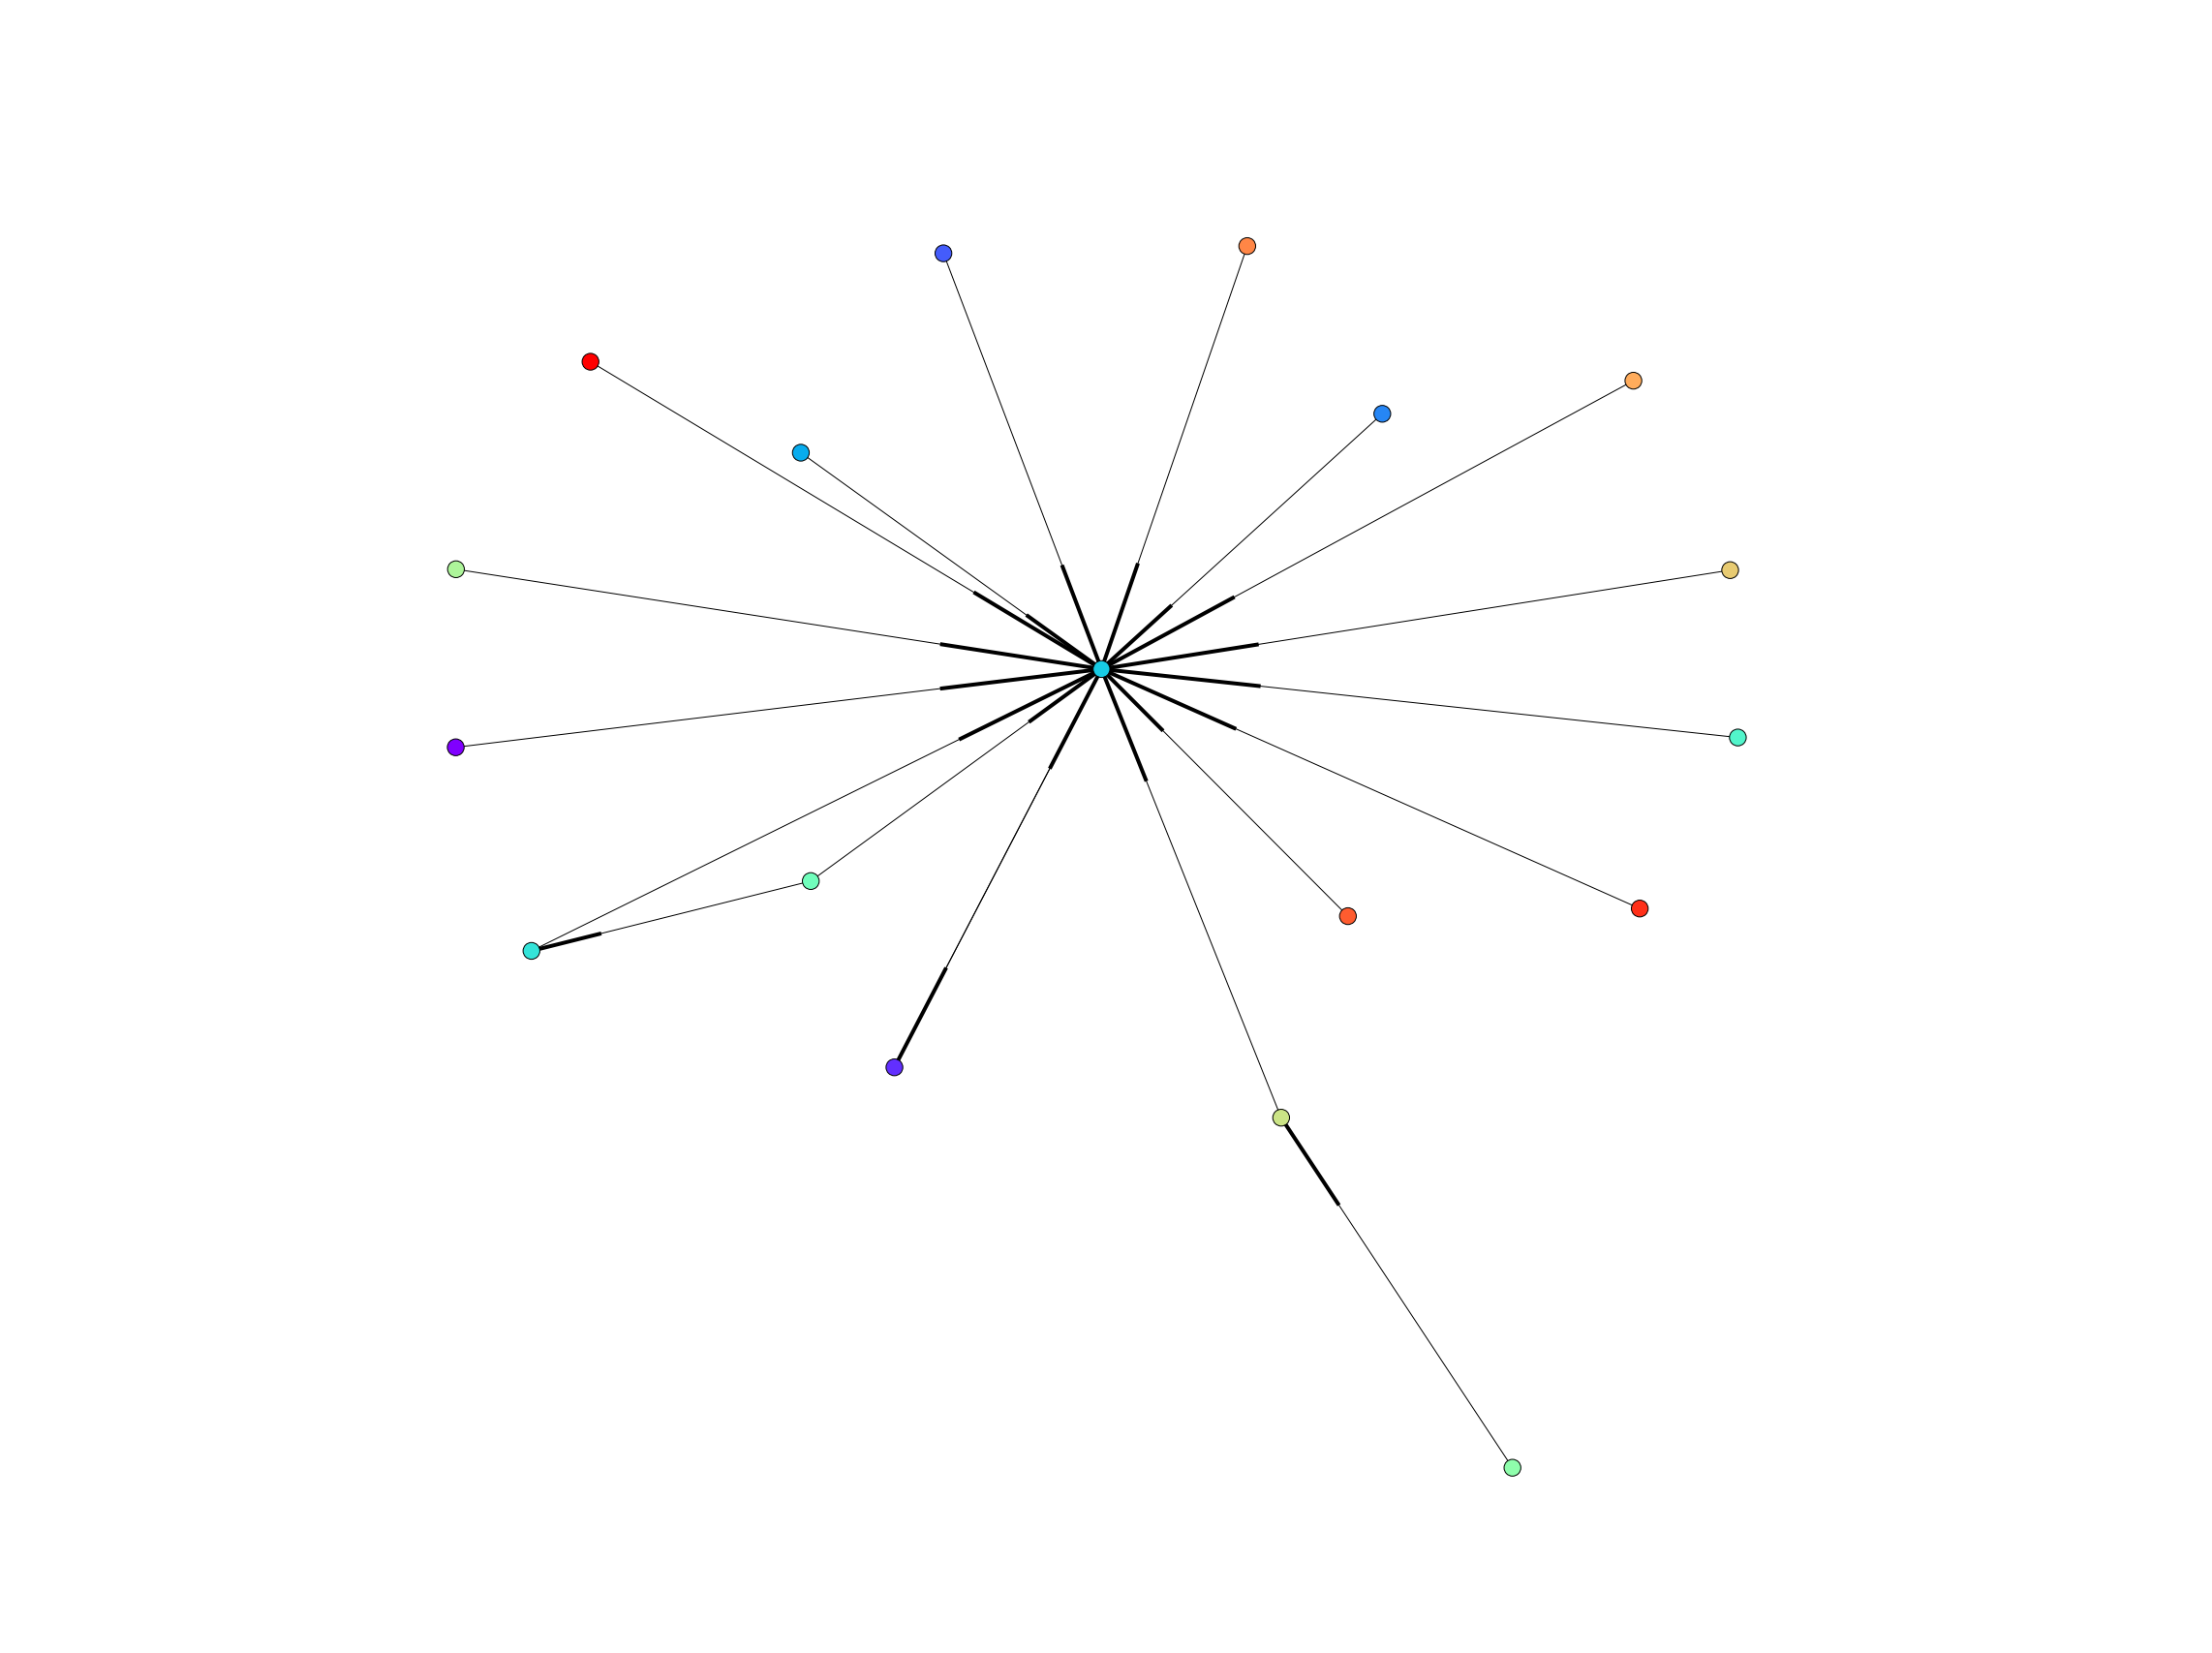
\includegraphics[width=0.5\textwidth ]{LowOPActivityGraph.png}
        \label{fig:rich_asthma}
    }
    \subfloat[]{
    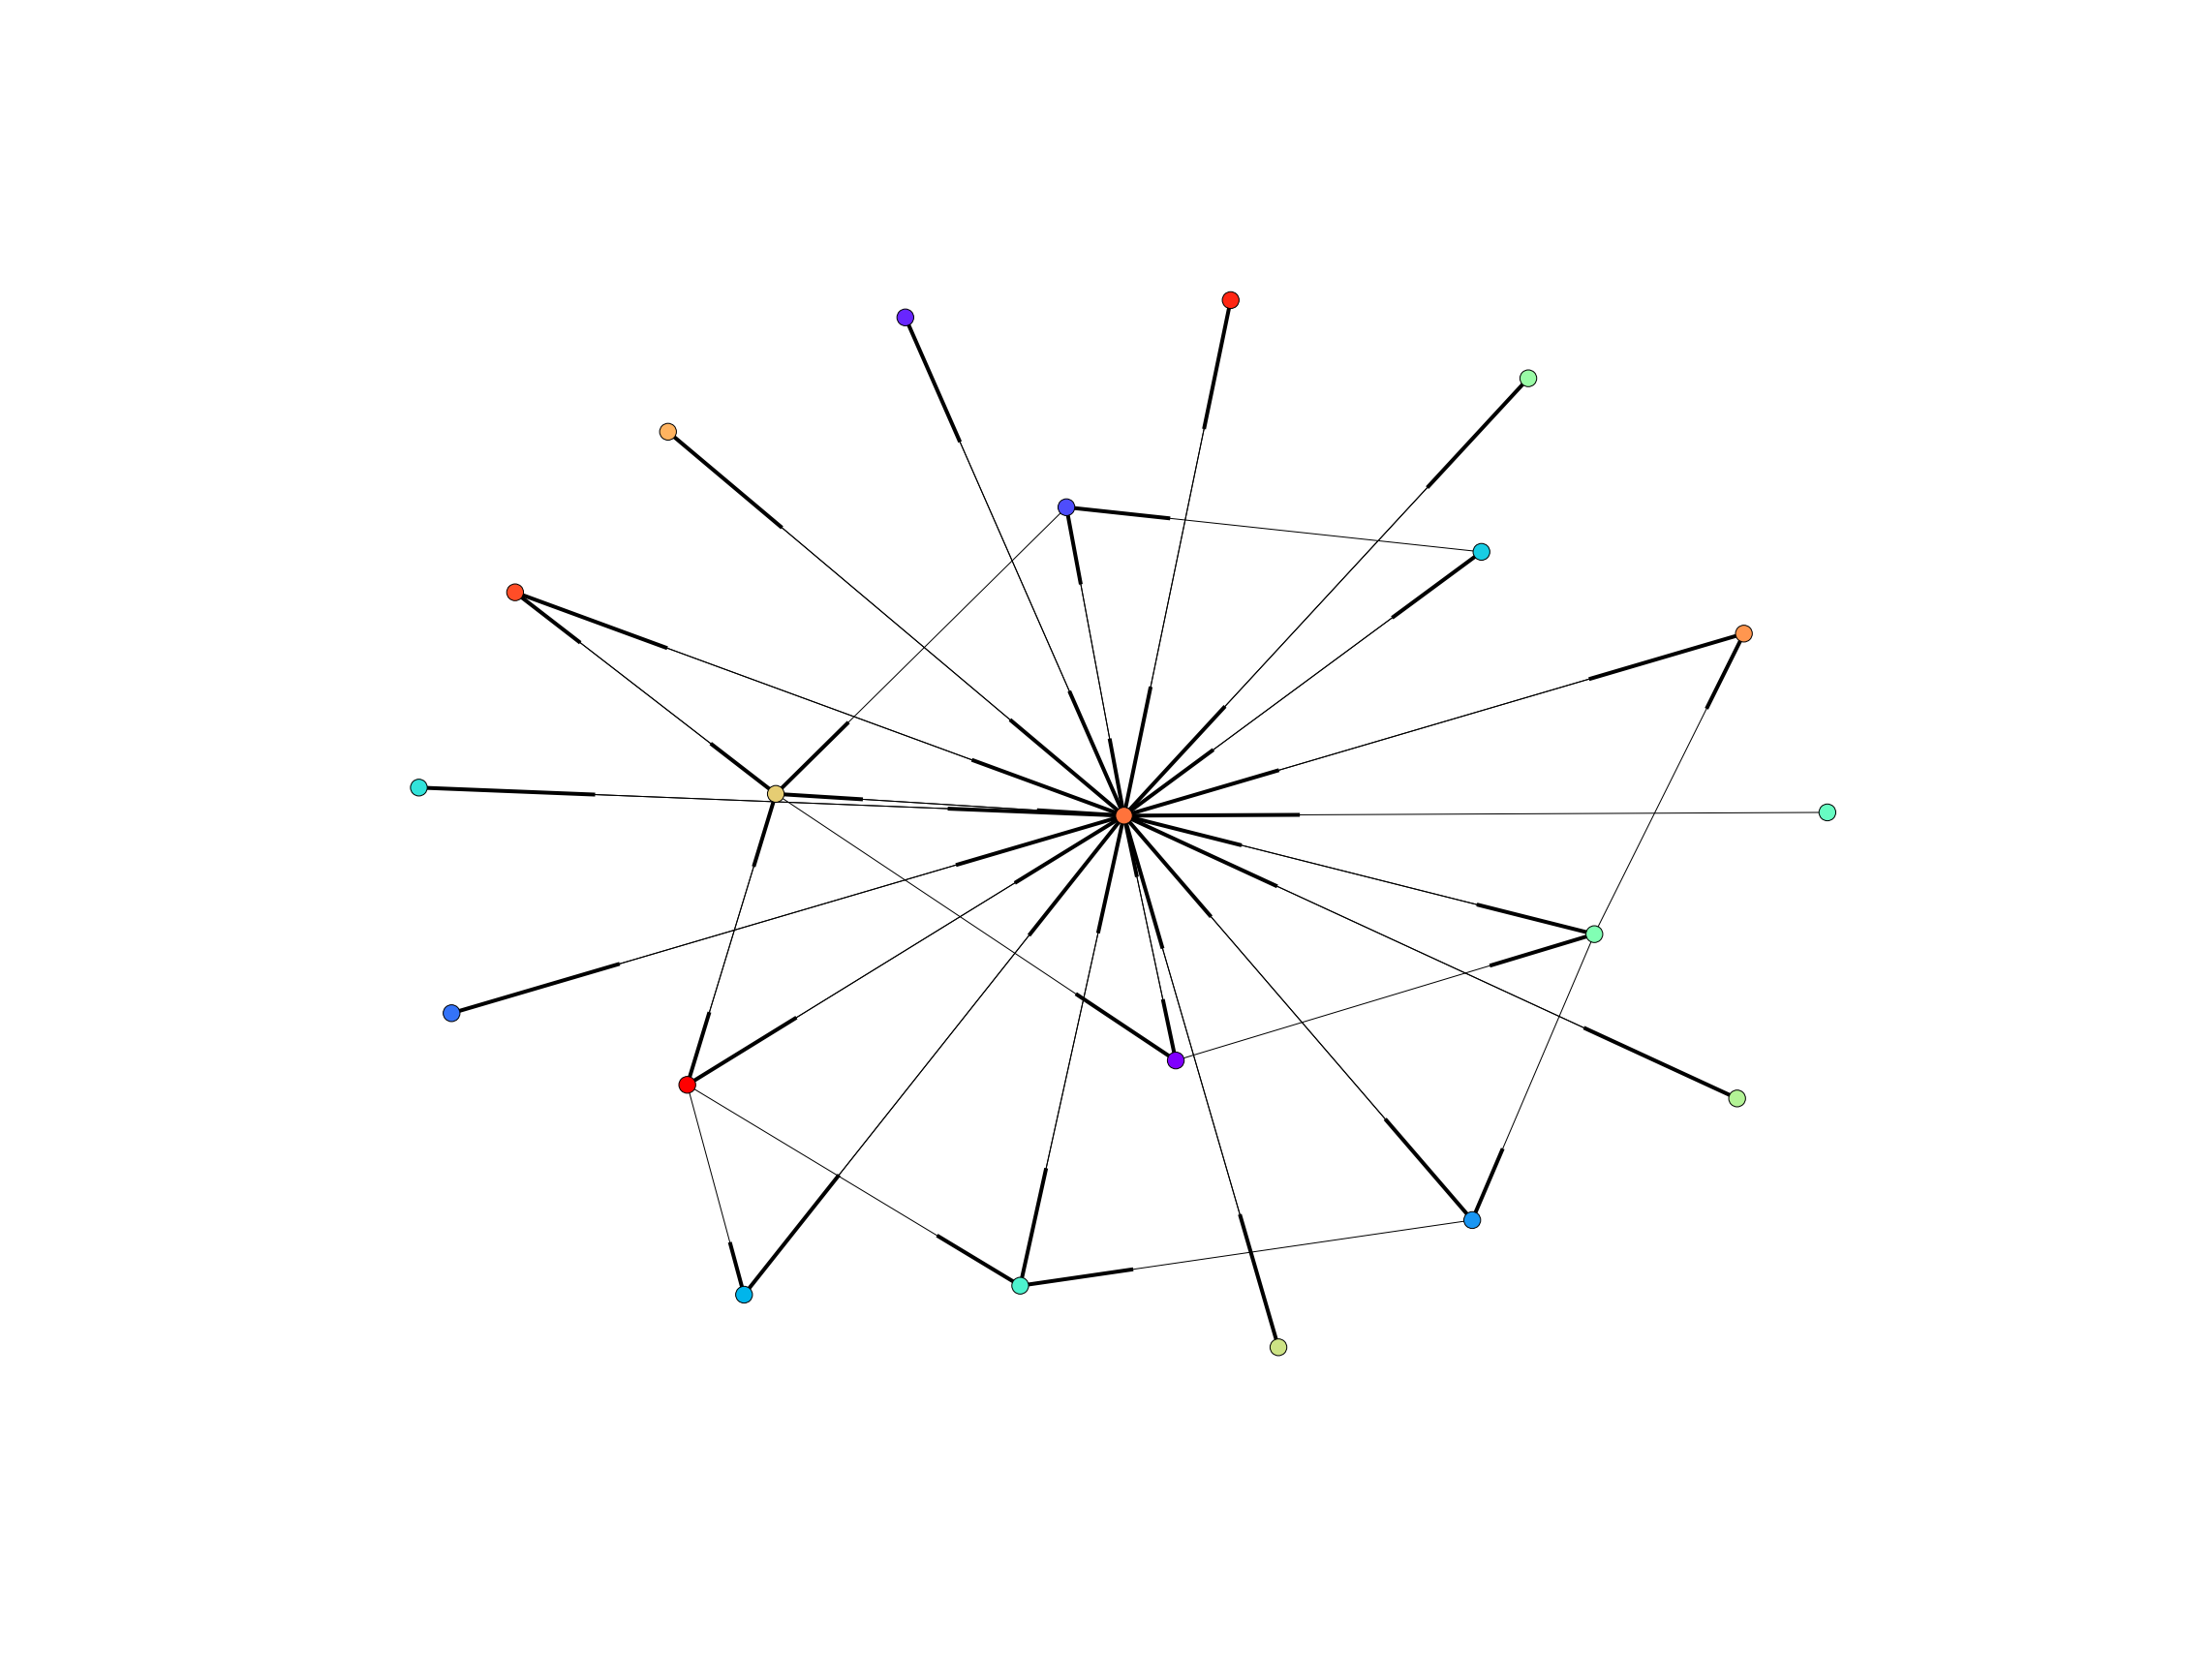
\includegraphics[width=0.5\linewidth ]{HighOPActivityGraph.png}
    \label{fig:rich_blf}
    }


    \subfloat[]{
        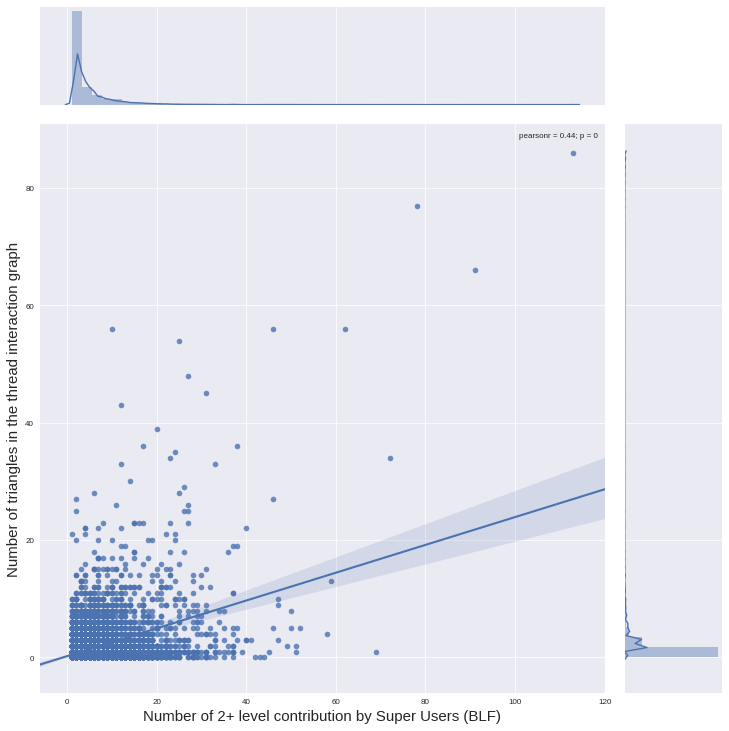
\includegraphics[width=0.5\linewidth ]{SUParticipationTriangles.png}
        \label{fig:rich_blf}
    }

    \caption{  }
\end{figure}

\section{Key takeaways, possible interventions}

